% DO NOT COMPILE THIS FILE DIRECTLY!
% This is included by the other .tex files.

\begin{frame}[t,plain]
\titlepage
\end{frame}

\begin{frame}
 \frametitle{MISP, comenzando desde un caso práctico}
 \begin{itemize}
         \item Durante un taller de análisis de malware en 2012, descubrimos que habíamos estado trabajando analizando el mismo malware.
         \item Quisimos compartir información de forma fácil y automatizada para así {\bf evitar la duplicación de trabajo}.
         \item Christophe Vandeplas (trabajando en el CERT del MINDEF Belga en aquel entonces) nos mostró su trabajo en una plataforma que luego se convertiría en MISP.
         \item Una primera versión de MISP fue utilizada por el MALWG y {\bf los comentarios de los usuarios} nos ayudaron a realizar mejoras en la plataforma.
         \item Actualmente MISP es {\bf un desarrollo impulsado por la comunidad}.
 \end{itemize}
\end{frame}

\begin{frame}
\frametitle{Acerca de CIRCL}
El Centro de Respuesta ante Emergencias Informáticas de Luxemburgo (CIRCL) es una iniciativa impulsada por el gobierno, diseñada para proveer una respuesta sistemática a incidentes y amenazas de seguridad informática.
\linebreak
\linebreak
CIRCL es el CERT del sector privado, municipios y entidades no gubernamentales en Luxemburgo y es operado por LHC g.i.e.
\end{frame}

\begin{frame}
\frametitle{MISP y CIRCL}
\begin{itemize}
\item CIRCL es conducido por el Ministerio de Economía y actúa como el CERT Nacional para el sector privado.
\item CIRCL lidera el desarrollo de MISP, la plataforma de código abierto de inteligencia de amenazas, que es utilizada por muchas comunidades militares o de inteligencia, empresas privadas, sector financiero, CERTs nacionales y fuerzas de seguridad (LEAs) en todo el mundo.
\item {\bf CIRCL opera múltiples comunidades de MISP, que a diario comparten información de inteligencia de amenazas (threat-intelligence)}.
\end{itemize}
        
\includegraphics{en_cef.png}
\end{frame}

\begin{frame}
\frametitle{¿Qué es MISP?}
\begin{itemize}
       \item MISP es una plataforma libre y de código abierto para el {\bf intercambio de información de amenazas}.
       \item Es una herramienta que {\bf recolecta} información proveniente de diferentes participantes, sus analistas, sus herramientas, fuentes de inteligencia, etc.
       \item Normaliza, {\bf correlaciona} y {\bf enriquece} la información.
       \item Permite {\bf colaborar} a los diferentes equipos y comunidades.
       \item {\bf Alimenta} las herramientas de seguridad y de los analistas con sus resultados.
\end{itemize}
\end{frame}

\begin{frame}
\frametitle{Desarrollo basado en comentarios de los usuarios}
\begin{itemize}
\item Existen muchos diferentes tipos de usuarios de plataformas de intercambio de información como MISP: 
        \begin{itemize}
                \item {\bf Analistas de Malware} dispuestos a compartir indicadores de compromiso con sus respectivos colegas.
                \item {\bf Analistas de Seguridad} buscando, validando y utilizando indicadores en seguridad operacional.
                \item {\bf Analistas de Inteligencia} recopilando información acerca de ciertos grupos de adversarios.
                \item {\bf Fuerzas de Seguridad} utilizando indicadores para dar soporte a casos de análisis forense digital (DFIR).
                \item {\bf Equipos de Análisis de Riesgos} dispuestos a saber más sobre nuevas amenazas, probabilidades e incidencias.
                \item {\bf Analistas de Fraude} dispuestos a compartir indicadores financieros para detectar fraudes.
        \end{itemize}
\end{itemize}
\end{frame}

\begin{frame}
\frametitle{Modelo de gobernabilidad de MISP}
\begin{center}
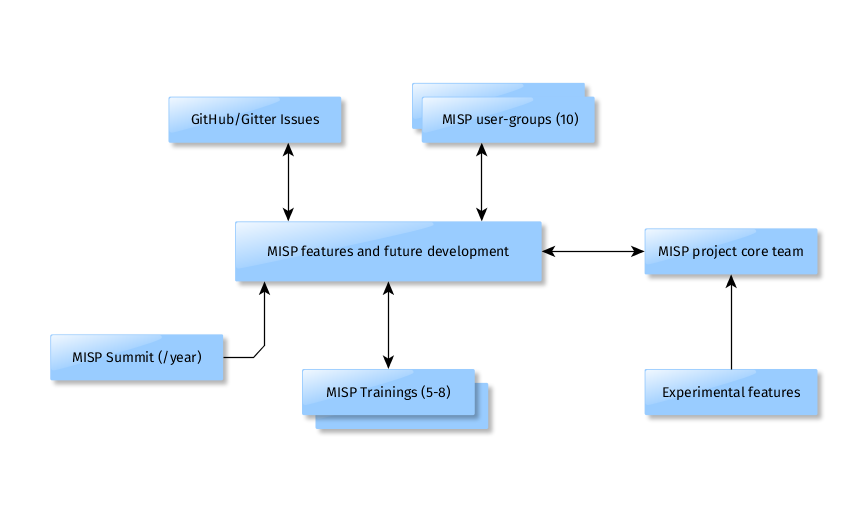
\includegraphics[scale=0.2]{governance.png}
\end{center}
\end{frame}

\begin{frame}
\frametitle{Múltiples objetivos según diferentes grupos de usuarios}
        \begin{itemize}
                \item Compartiendo indicadores para la {\bf detección}.
                        \begin{itemize}
                                \item '¿Existen sistemas infectados en mi infraestructura o en las redes que opero?'
                        \end{itemize}
                \item Compartiendo indicadores para {\bf bloquear}.
                        \begin{itemize}
                                \item 'Utilizo estos indicadores para bloquear el acceso o redireccionar el tráfico.'
                        \end{itemize}
                \item Compartiendo indicadores para {\bf realizar actividades de inteligencia}.
                        \begin{itemize}
                                \item 'Recopilando información acerca de campañas y ataques. ¿Están relacionados? ¿Quién me tiene como objetivo? ¿Quiénes son los adversarios?'
                        \end{itemize}
                \item $\rightarrow$ Estos objetivos pueden ser contradictorios (p. ej. Los falsos-positivos tienen diferentes impactos)
        \end{itemize}
\end{frame}

\begin{frame}
 \frametitle{Comunidades utilizando MISP}
 \begin{itemize}
	 \item Las comunidades son grupos de usuarios que comparten un conjunto objetivos o valores comunes.
	 \item CIRCL opera múltiples instancias de MISP con una gran cantidad de usuarios (más de 1200 organizaciones con más de 4000 usuarios).
         \item {\bf Grupos de confianza} operando comunidades de MISP en modo aislado (air-gapped) o parcialmente conectados.
	 \item {\bf Sector financiero} (bancos, Centros de Análisis e Intercambio de Información (ISACs), organizaciones de procesamiento de pagos) utilizan MISP como mecanismo de intercambio.
	 \item {\bf Organizaciones internacionales y militares} OTAN, CSIRTs militares, CERTs, ...
	 \item {\bf Proveedores de Seguridad} operando sus propias comunidades o interconectados con otras comunidades.
         \item {\bf Comunidades temáticas} creadas para abordar problemáticas específicas (COVID-19 MISP) 
 \end{itemize}
\end{frame}

\begin{frame}
\frametitle{Las dificultades de compartir información}
        \begin{itemize}
                \item Las dificultades de compartir información no suelen ser problemas de índole tecnológico, en general se deben a las {\bf interacciones sociales} (p. ej. {\bf confianza}).
                \item Restricciones legales\footnote{\url{https://www.misp-project.org/compliance/}}
                        \begin{itemize}
                                \item "Nuestro marco legal no nos permite compartir información."
                                \item "El riesgo de filtraciones de información es muy alto y riesgoso para nuestra organización y nuestros socios."
                        \end{itemize}
                \item Restricciones prácticas
                        \begin{itemize}
                                \item "No tenemos información para compartir."
                                \item "No tenemos tiempo para procesar o contribuir con indicadores."
                                \item "Nuestro modelo de clasificación no se ajusta al modelo de MISP."
                                \item "Las herramientas para intercambio de información están asociadas a un formato específico, nosotros utilizamos otro."
                        \end{itemize}
        \end{itemize}
\end{frame}


\begin{frame}
        \frametitle{Vista general del Proyecto MISP}
        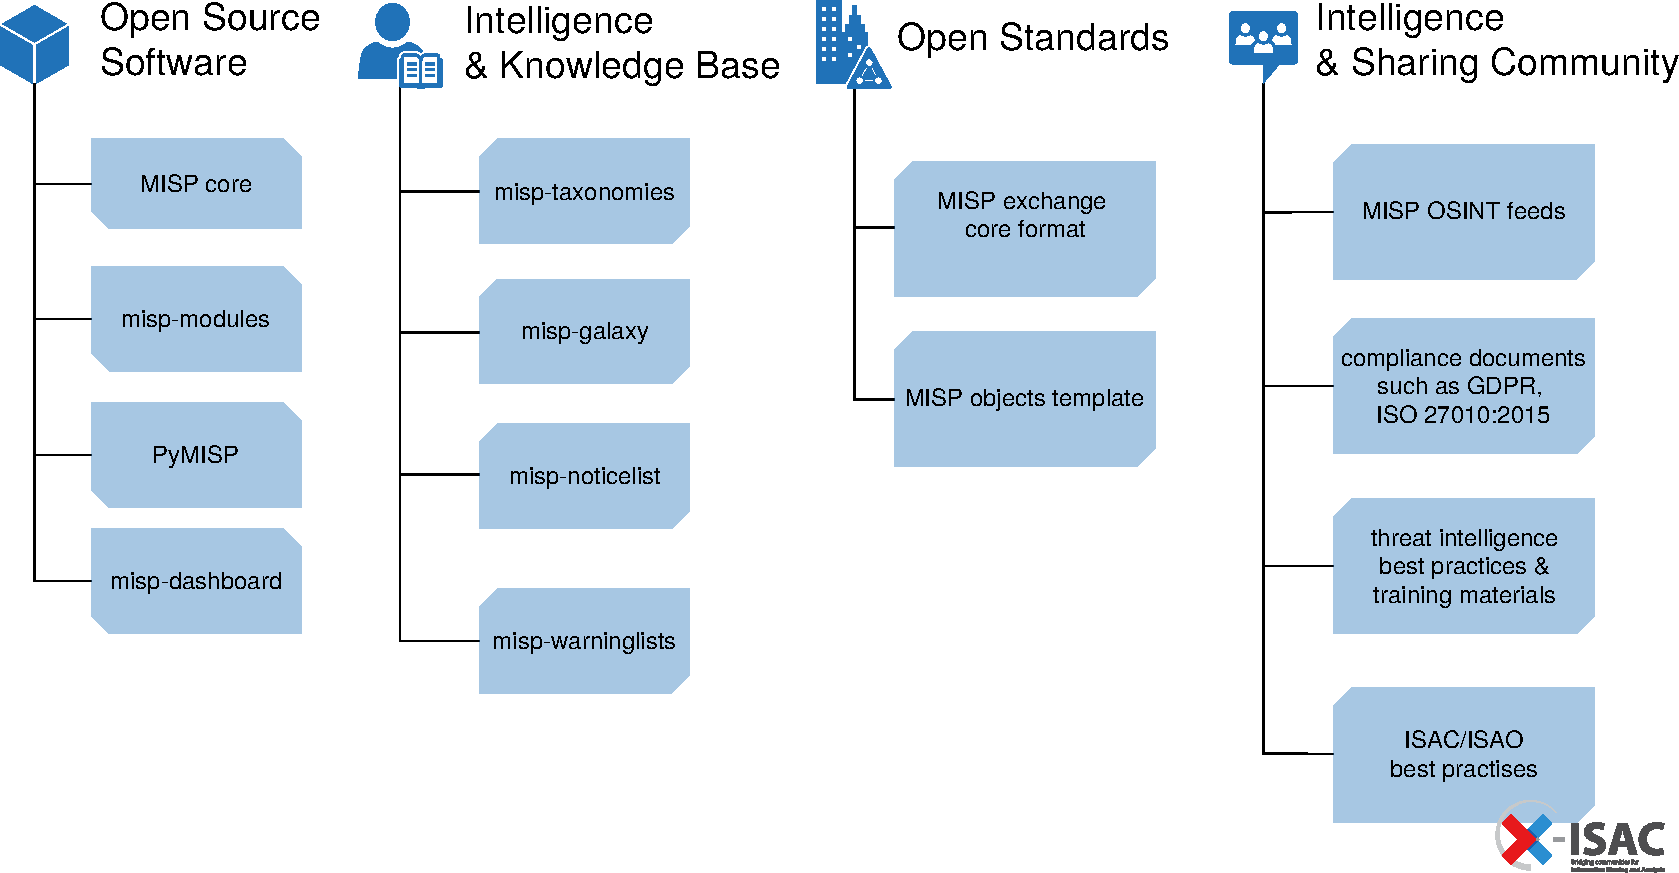
\includegraphics[scale=0.35]{misp-overview-simplified.pdf}
\end{frame}

\begin{frame}
\frametitle{Compartiendo en MISP}
    \begin{itemize}
        \item Compartiendo vía listas de distribución - {\bf Grupos de intercambio} (sharing groups)
        \item {\bf Delegación} para intercambio de información pseudo-anonimizada
        \item {\bf Propuestas} y {\bf Eventos extendidos} para compartir información en forma colaborativa
        \item Sincronización, Fuentes (feeds), intercambio aislado (air-gapped)
        \item {\bf Filtros de intercambio } definidos por el usuario para todos los métodos mencionados anteriormente
        \item {\bf Almacenamiento en caché} para búsquedas rápidas en grandes volúmenes de datos
        \item Soporte de múltiples instancias de MISP para enclaves internas
    \end{itemize}
\end{frame}

\begin{frame}
\frametitle{Gestión de la calidad de la Información}
    \begin{itemize}
        \item Información correlacionada
        \item Ciclo de retroalimentación de detecciones vía {\bf Avistamientos} (Sightings)
        \item {\bf Gestión de falsos positivos} vía el sistema de alertas (warninglists)
        \item Sistema de {\bf enriquecimiento} vía MISP-modules
        \item Sistema de {\bf flujos de trabajo} para revisar y controlar la información que se publica
        \item {\bf Integraciones} con un gran número de herramientas y formatos
        \item {\bf API} flexible y soporte de {\bf librerías} tales como PyMISP para facilitar la integración
        \item {\bf Líneas de tiempo} (timelines) para dotar a la información de un marco temporal
        \item Cadena completa de la {\bf gestión del ciclo de vida de indicadores}
    \end{itemize}
\end{frame}

\begin{frame}
        \frametitle{Conclusión}
        \begin{itemize}
                \item {\bf Las prácticas de intercambio de información vienen con su uso} y con el ejemplo (p. ej. aprender mediante la imitación de la información compartida).
                \item MISP es sólo una herramienta. Lo que importa son sus prácticas de intercambio. La herramienta debería darle soporte de la manera más transparente posible.
                \item Permitir a los usuarios customizar MISP para satisfacer las necesidad de los casos de uso de su comunidad.
                \item El proyecto MISP combina código abierto, estándares abiertos, mejores prácticas y comunidades para convertir el intercambio de información en una realidad.
        \end{itemize}
\end{frame}


